\subsubsection{Mapping Properties of Simple Functions}
Similar to how functions with real variables map values to a different set of values, complex functions do the same. The main difference is that with complex functions we're mapping a 2 dimensional set of inputs to a 2 dimensional set of outputs.
\[
w=f(z)=u+iv
\]
We define $z\in \mathcal{S}$ the image of $\mathcal{S}$ under $w$.\\
Some common mappings:
\begin{itemize}
    \item The identity map
    \begin{align*}
        &w=f(z)=z\\
        &\eqnsystem{u=x\\ v=y}
    \end{align*}
    \item Translation by $z_0$
    \begin{align*}
        &w=f(z)=z+z_0\\
        &\eqnsystem{u=x+x_0\\ v=y+y_0}
    \end{align*}
    \item Stretching ($a>1$) or contraction ($a<1$)
    \begin{align*}
        &w=f(z)=az=are^{i\varphi},\ a\in\R\\
        &\eqnsystem{u=ax\\ v=ay}
    \end{align*}
    \item Rotation by $\varphi_0$
    \begin{align*}
        &w=f(z)=e^{i\varphi_0}z=e^{i(\varphi+\varphi_0)}
    \end{align*}
\end{itemize}
Using these basic mapping principles we are able to lay the foundation for some more complicated mappings.\\
Ex: Find the image of $S=\brcurly{|z-1|\geq1}$ under the mapping $f(z)=\frac{1}{z}$\\
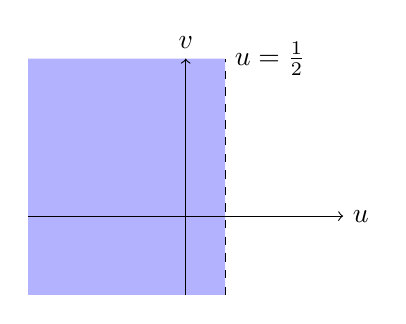
\begin{tikzpicture}
    % Region u <= 1/2
    \fill[blue!30, domain=-2:0.5, variable=\x]
        (-2, -1) -- plot ({\x}, {2}) -- (0.5, -1) -- cycle;

    % Axes
    \draw[->] (-2,0) -- (2,0) node[right] {$u$};
    \draw[->] (0,-1) -- (0,2) node[above] {$v$};
    
    % Dashed line u = 1/2
    \draw[dashed] (0.5, -1) -- (0.5, 2) node[right] {$u=\frac{1}{2}$};
\end{tikzpicture}

\begin{align*}
    &z=\frac{1}{w}=\frac{1}{u+iv}=\frac{u-iv}{u^2+v^2}\\
    &x=\frac{u}{u^2+v^2}\\
    &y=-\frac{v}{u^2+v^2}\\
    &|z-1|\geq1\Ra\brvertical{\frac{1}{w}-1}\geq1\\
    &\frac{1-w}{w}\geq1\\
    &|1-w|\geq|w|\\
    &|1-w|^2\geq|w|^2\\
    &(1-u)^2+v^2\geq u^2+v^2\\
    &-2u+1\geq 0\\
    &u\leq\frac{1}{2}\\
    &S'=\brcurly{u\leq\frac{1}{2}}
\end{align*}


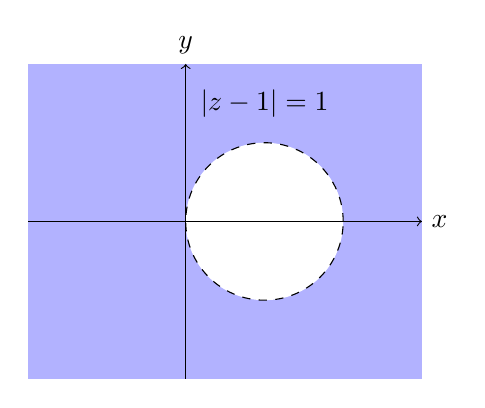
\begin{tikzpicture}
    % Background (Blue)
    \fill[blue!30] (-2,-2) rectangle (3,2);

    % Region |z-1| >= 1
    \fill[blue!30, domain=-1:1, variable=\x]
        (-2, 0) -- plot ({1+\x}, {sqrt(1 - \x*\x)}) -- (2, 0) -- cycle;
    \fill[blue!30, domain=-1:1, variable=\x]
        (-2, 0) -- plot ({1+\x}, {-sqrt(1 - \x*\x)}) -- (2, 0) -- cycle;

    % Circle (White, Dashed)
    \draw[fill=white, dashed] (1, 0) circle (1);

    % Label: |z-1| = 1
    \node at (1, 1.5) {$|z-1|=1$};

    % Axes
    \draw[->] (-2,0) -- (3,0) node[right] {$x$};
    \draw[->] (0,-2) -- (0,2) node[above] {$y$};
\end{tikzpicture}

Ex2: Find the image of $S=\brcurly{x\leq1}$ under the mapping $f(z)=\frac{1}{z}$

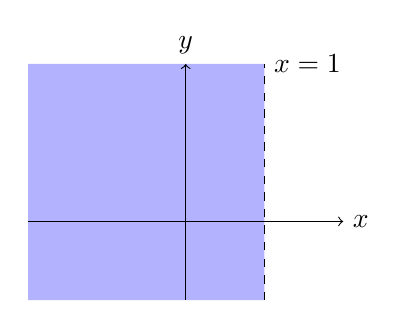
\begin{tikzpicture}
    % Region x <= 1
    \fill[blue!30, domain=-2:1, variable=\x]
        (-2, -1) -- plot ({\x}, {2}) -- (1, -1) -- cycle;

    % Axes
    \draw[->] (-2,0) -- (2,0) node[right] {$x$};
    \draw[->] (0,-1) -- (0,2) node[above] {$y$};
    
    % Dashed line x = 1
    \draw[dashed] (1, -1) -- (1, 2) node[right] {$x=1$};
\end{tikzpicture}
\begin{align*}
    &z=\frac{1}{w}=\frac{1}{u+iv}=\frac{u-iv}{u^2+v^2}\\
    &x=\frac{u}{u^2+v^2}\\
    &x\leq1\Ra \frac{u}{u^2+v^2}\leq1\Ra u^2+v^2\geq u\\
    &(u-\tfrac{1}{2})^2+v^2\geq\tfrac{1}{4}
\end{align*}

% create a new tikzpicture of the circle |z-\frac{1}{2}|>=1/2
\begin{tikzpicture}
    % Background (Blue)
    \fill[blue!30] (-2,-2) rectangle (3,2);

    % Region |z-1| >= 1
    \fill[blue!30, domain=-1:1, variable=\x]
        (-2, 0) -- plot ({1+\x}, {sqrt(1 - \x*\x)}) -- (2, 0) -- cycle;
    \fill[blue!30, domain=-1:1, variable=\x]
        (-2, 0) -- plot ({1+\x}, {-sqrt(1 - \x*\x)}) -- (2, 0) -- cycle;

    % Circle (White, Dashed)
    \draw[fill=white, dashed] (1, 0) circle (1);

    % Label: |z-1| = 1
    \node at (1, 1.5) {$|z-\tfrac{1}{2}|=\tfrac{1}{2}$};

    % Axes
    \draw[->] (-2,0) -- (3,0) node[right] {$x$};
    \draw[->] (0,-2) -- (0,2) node[above] {$y$};
\end{tikzpicture}
We see from the previous two examples that circles map to lines and lines map to circles. Let's see why this is the case.
\begin{align*}
    &a(x^2+y^2)+bx+cy+d=0\\
    &a|z|^2+b\frac{z+\bar{z}}{2}+c\frac{z-\bar{z}}{2i}+d=0
\end{align*}
In the case where $a=0$, we have a line. In the case where $a\neq0$, we have a circle.
\begin{align*}
    &w=\frac{1}{z}\Ra z=\frac{1}{w}\\
    &z\bar{z}=|z|^2=\frac{1}{|w|^2}=\frac{1}{w\bar{w}}\\
    &a\frac{1}{w\bar{w}}+b\frac{z+\bar{z}}{2}+c\frac{z-\bar{z}}{2i}+d=0\\
    &a\frac{1}{w\bar{w}}+\frac{b}{2}\brround{\frac{1}{w}+\frac{1}{\bar{w}}}+\frac{c}{2i}\brround{\frac{1}{w}-\frac{1}{\bar{w}}}+d=0\\
    &a+\frac{b}{2}\brround{w+\bar{w}}+\frac{c}{2i}\brround{w-\bar{w}}+d\brround{w\bar{w}}=0\\
\end{align*}
If we have a linear transformation of the form $az+b$ it corresponds to the scaling and translation of the set only. A line will map to a line and a circle will map to a circle.\\
We can combine this with the $w=\frac{1}{z}$ transformation property to get a more general transformation. We call this the \textit{Mobius transformation}:
$$f(z)=\frac{az+b}{cz+d}=\frac{a}{c}+\frac{b-\tfrac{ad}{c}}{cz+d}$$

Ex: Find the mapping of $f(z)=\frac{1}{z+1}$ on the set $S=\brcurly{\Re(z)>0}$ 
\begin{align*}
    &u+iv=\frac{1}{x+1+iy}\Ra x+1+iy=\frac{1}{u+iv}\\
    &x+1=\frac{u}{u^2+v^2}\\
    &x>0\Ra x+1>1\\
    &\frac{u}{u^2+v^2}>1\Ra u>u^2+v^2\\
    &u^2+v^2-u+\frac{1}{4}<\frac{1}{4}\\
    &\brround{u-\frac{1}{2}}^2+v^2<\frac{1}{4}\\
    &S'=\brcurly{w=u+iv\Bigg\vert\brround{u-\frac{1}{2}}^2+v^2<\bfrac{1}{2}^2}
\end{align*}

Ex2: Find the mapping of $f(z)=\frac{z-i}{z+i}$ on $S=\brcurly{|z|<3}$
\begin{align*}
    &wz+iw=z-i\Ra z(w-1)=-i-iw\Ra z=\frac{i(w+1)}{1-w}\\
    &|z|=\frac{|w+1|}{|w-1|}<3\\
    &|w+1|<3|w-1|\Ra |w+1|^2<9|w-1|^2\\
    &(u+1)^2+v^2<9(u-1)^2+9v^2\\
    &u^2+2u+1+v^2<9u^2-18u+9+9v^2\\
    &0<8u^2-20u+8+8v^2\Ra 0<u^2-\frac{5}{2}u+1+v^2\\
    &\frac{9}{16}<u^2-\frac{5}{2}u+\frac{25}{16}+v^2\\
    &\frac{9}{16}<\brround{u-\frac{5}{4}}^2+v^2\\
    &S'=\brcurly{w=u+iv\Bigg\vert\brround{u-\frac{5}{4}}^2+v^2>\bfrac{3}{4}^2}
\end{align*}


Ex3: Find the mapping of $f(z)=-2z^5$ on $S=\brcurly{|z|<1,0<\Arg(z)<\frac{\pi}{2}}$
\begin{align*}
    &z^5=-\frac{w}{2}\Ra |z|^5=\frac{|w|}{2}<1\Ra |w|<2\\
    &5\arg(z)=\arg(w)\pm\pi \\
    &0<\arg(w)\pm\pi <\frac{5\pi}{2}\\
    &-\pi<\arg(w)<\frac{3\pi}{2}\\
    &S'=\brcurly{|w|<2}
\end{align*}